
\subsection{Counter examples for the invalid cases}

    For each case where reordering is not safe to do, we also show counter examples of programs where new observable behaviors are introduced.
    This additionally potrays additional proof of the validity of our approach. 

    For all the examples we show here, we only show the ordering relations that are important to observe. 
    Putting all the relations among different events in the example will result in confusion, hence we avoid doing so. 

    \paragraph{Reads to same memory where $e$ is of type $sc$ while $d$ is of either $uo/sc$}
        
        The following example involves two reads to the same memory and a write. 
        
        \begin{figure}[H]
            \centering
            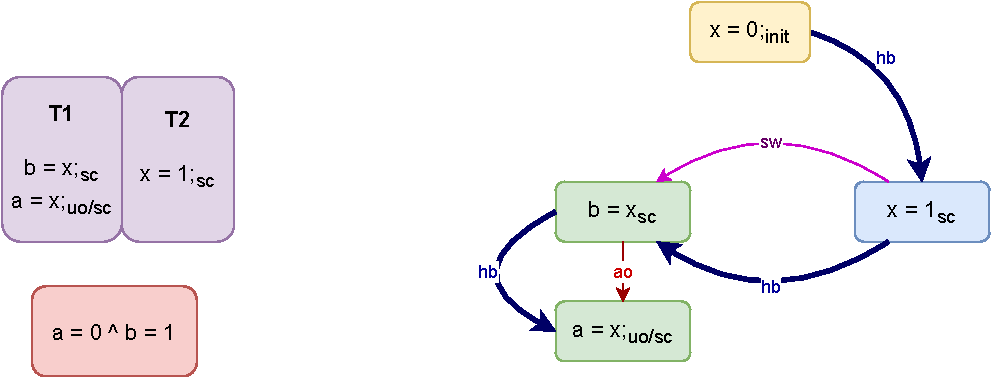
\includegraphics[scale=0.7]{InstructionReordering/Example1(Rsc-Ruo,sc).pdf}
            \caption{Case where a = 0 , b = 1 is invalid due to Coherent Reads}
        \end{figure}

        The figure on the left above shows an example of a candidate where the case of reads in the red box is not possible. 
        The figure on the right shows the Candidate Execution of such a case. 
        Observations:
        \begin{itemize}
            \item We can infer from the Candidate Execution that $\reln{\{x=0_{init}\}}{hb}{\reln{\{x=1_{sc}\}}{hb}{\{a=x_{uo/sc}\}}}$.
            \item By the Axiom \ref{CoRe}, it is not possible for $a$ to read the value of $0$ as $x$ due to the intervening write whiCh changes $x$ to $1$.  
            \item This inference does not rely upon the access mode of the read $a$. 
        \end{itemize}
        
        \begin{figure}[H]
            \centering
            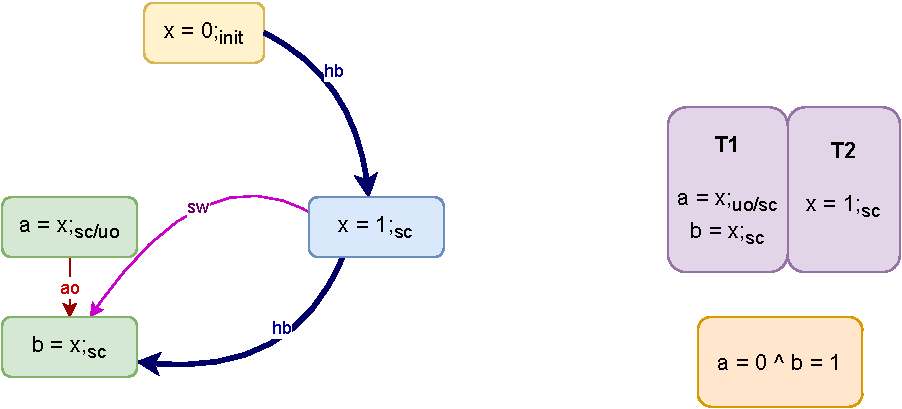
\includegraphics[scale=0.7]{InstructionReordering/Example1R(Rsc-Ruo,sc).pdf}
            \caption{Case where the reads are reordered and a = 0 , b = 1 is valid}
        \end{figure}

        The figure on the right shows the program after reordering the two reads in $T1$, where the case of reads in the orange box is possible. 
        The figure on the left shows the Candidate Execution of such a case. 

        Observations:
        \begin{itemize}
            \item From the Candidate Execution, we can infer $\neg\reln{\{x=0_{init}\}}{hb}{\reln{\{x=1_{sc}\}}{hb}{\{a=x_{uo/sc}\}}}$
            \item We can also infer that $\reln{\{x=0_{init}\}}{hb}{\{a=x_{uo/sc}\}}$    
            \item Since none of the Axioms disallow the above pattern, $a$ is allowed to read the value of $x$ to be $0$.
            \item Hence, the reordering of the two reads is invalid. 
        \end{itemize}
%---------------------------------------------------------------------------------------------------------------------------------------
    \paragraph{Reads to non-equal range  of memory where $e$ is of type $sc$ while $d$ is of either $uo/sc$}

%---------------------------------------------------------------------------------------------------------------------------------------    
    \paragraph{A Read $e$ of type $sc$ followed by a Write of either $uo/sc$}
        
        The following is an example of a program with a sequentially consistent read followed by a write of any type. 
        \begin{figure}[H]
            \centering
            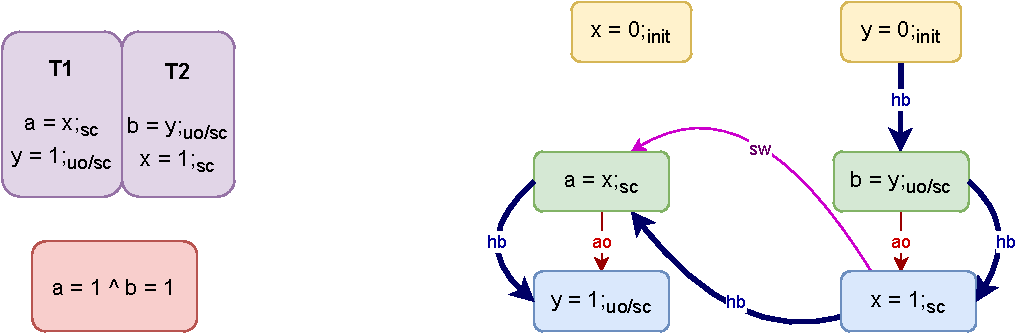
\includegraphics[scale=0.7]{InstructionReordering/Example3(Rsc-Wuo,sc).pdf}
            \caption{Case where a = 1 and b = 1 is invalid due to Coherent Reads.}
        \end{figure}
        The figure on the left above shows an example of a candidate where the case of reads in the red box is not possible. 
        The figure on the right shows the Candidate Execution of such a case. 
        Observations:
        \begin{itemize}
            \item From the Candidate Execution, we can infer $\reln{b=y_{uo/sc}}{hb}{y=1_{uo/sc}}$
            \item By Axiom \ref{CoRe}, $b$ cannot read the value of $1$ as $y$. 
            \item This inference was due to $\reln{x=1_{sc}}{hb}{a=x{sc}}$
        \end{itemize}

        \begin{figure}[H]
            \centering
            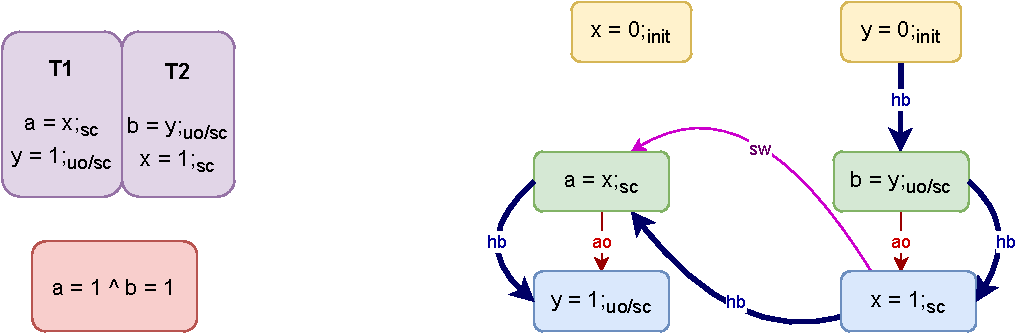
\includegraphics[scale=0.7]{InstructionReordering/Example3(Rsc-Wuo,sc).pdf}
            \caption{Case where events of T1 are reordered, resulting in  a = 1 and b = 1 to be valid.}
        \end{figure}
        The figure on the right above shows the program after reordering the two events in $T1$ where case of reads in the orange box is possible. 
        The figure on the left shows the Candidate Execution of such a case. 
        Observations:
        \begin{itemize}
            \item From the Candidate Execution, we can infer $\neg\reln{b=y_{uo/sc}}{hb}{y=1_{uo/sc}}$
            \item Since there is no $\stck{_{hb}}$ relation among the above two events, $b$ can read the value of $y$ as $1$.
        \end{itemize}

%--------------------------------------------------------------------------------------------------------------------------------------        
    \paragraph{A Read $e$ of type $uo$ followed by a write $d$ of type $sc$}

        For this we can use the same example for the previous part (tag figure of example), where we just reorder $T2$'s events.
        \begin{figure}[H]
            \centering
            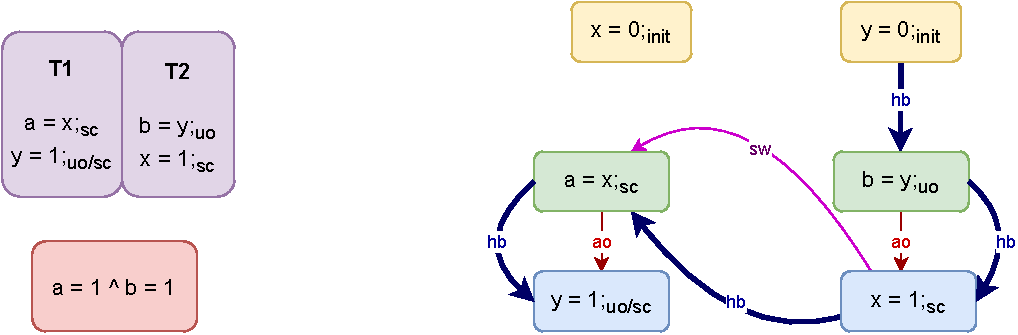
\includegraphics[scale=0.7]{InstructionReordering/Example4(Ruo-Wsc).pdf}
            \caption{Case where a = 1 and b = 1 is invalid due to Coherent Reads.}
        \end{figure}

        \begin{figure}[H]
            \centering
            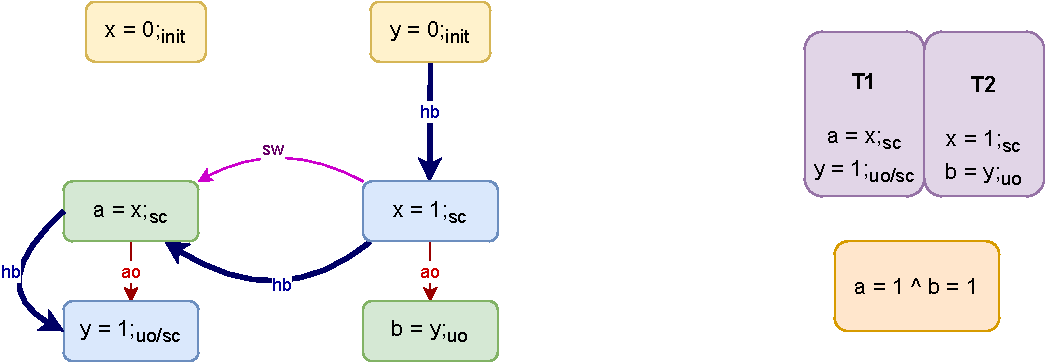
\includegraphics[scale=0.7]{InstructionReordering/Example4R(Ruo-Wsc).pdf}
            \caption{Case where events of T2 are reordered, resulting in  a = 1 and b = 1 to be valid.}
        \end{figure}

%---------------------------------------------------------------------------------------------------------------------------------------
        
    \paragraph{A Write $e$ followed by a Read $d$ both of type $sc$}
        
        A counter example for this is different. It is not the Observable Behavior we are concerned with that is introduced, but that which is allowed but creates a $\stck{_{hb}}$ cycle. The following example is as such:
        \begin{figure}[H]
            \centering
            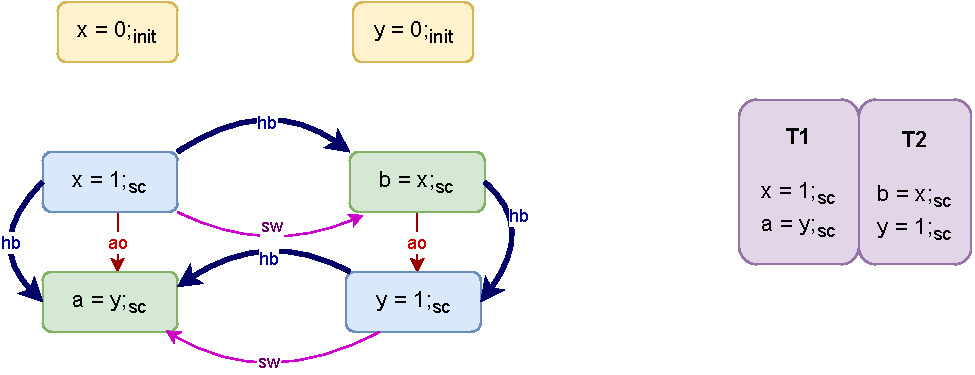
\includegraphics[scale=0.7]{InstructionReordering/Example5(Wsc-Rsc).pdf}
            \caption{Case where a = 1 and b = 1 is valid and no happens-before cycles}
        \end{figure}

        After reordering the two events of $T1$ in the above example, the same observable behavior holds, but has a cycle introduced. One might think that simply discarding that execution would do. But this would mean discarding $\stck{_{hb}}$ relations also, which would require more information to infer which relations are going to create such cycles and which are not. Since we place no assumptions on these relations, but that any happens-before relation other than the one we remove explicitly be reordering are all possible. Hence, the following reordered program outcome is something we do not risk to allow.

        \begin{figure}[H]
            \centering
            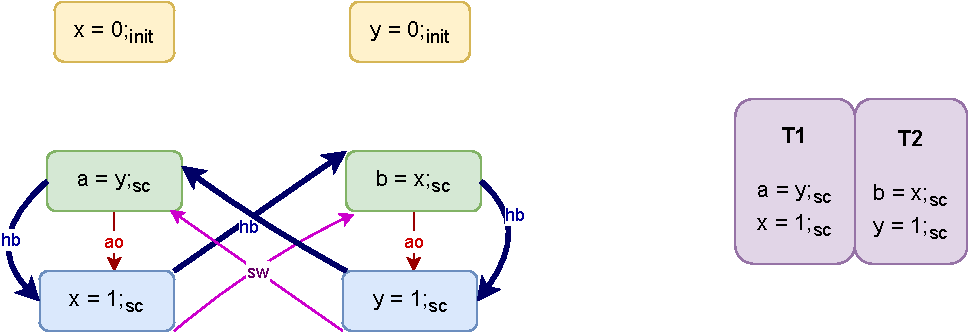
\includegraphics[scale=0.7]{InstructionReordering/Example5R(Wsc-Rsc).pdf}
            \caption{Case where a = 1 and b = 1 is creates a happens-before cycle}
        \end{figure}

        Observation:
        \begin{itemize}
            \item From the read values we can infer that the Candidate Execution should have $\reln{x=1_{sc}}{hb}{a=x_{sc}}$ and $\reln{y=1_{sc}}{hb}{a=y_{sc}}$.
            \item The above relations create the cycle $\reln{a=y_{sc}}{hb}{\reln{x=1_{sc}}{hb}{\reln{a=x_{sc}}{hb}{\reln{y=1_{sc}}{hb}{a=y_{sc}}}}}$.
            \item This execution is invalid. 
        \end{itemize}

%---------------------------------------------------------------------------------------------------------------------------------------

    \paragraph{A Write $e$ of type $uo/sc$ followed by a Write $d$ of type $sc$}
        
        The following example shows a program with a thread having a write of any access mode($uo/sc$) followed by a write of type $sc$.
        \begin{figure}[H]
            \centering
            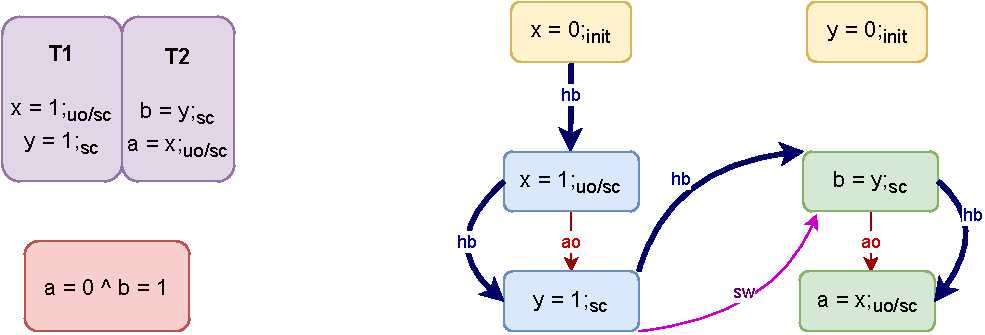
\includegraphics[scale=0.7]{InstructionReordering/Example7(Wuo,sc-Wsc).pdf}
            \caption{Case where a = 0 and b = 1 is invalid due to Coherent Reads.}
        \end{figure}
        The figure on the left above shows an example of a candidate where the case of reads in the red box is not possible. 
        The figure on the right shows the Candidate Execution of such a case. 
        Observations:
        \begin{itemize}
            \item From the Candidate Execution, we can infer $\reln{x=0_{init}}{hb}{\reln{x=1_{uo/sc}}{hb}{a=x_{uo/sc}}}$
            \item By Axiom \ref{CoRe}, the read of $a$ cannot have the value of $x$ read as $0$. 
            \item This inference was due to $\reln{y=1_{sc}}{hb}{b=y_{sc}}$.
        \end{itemize}

        \begin{figure}[H]
            \centering
            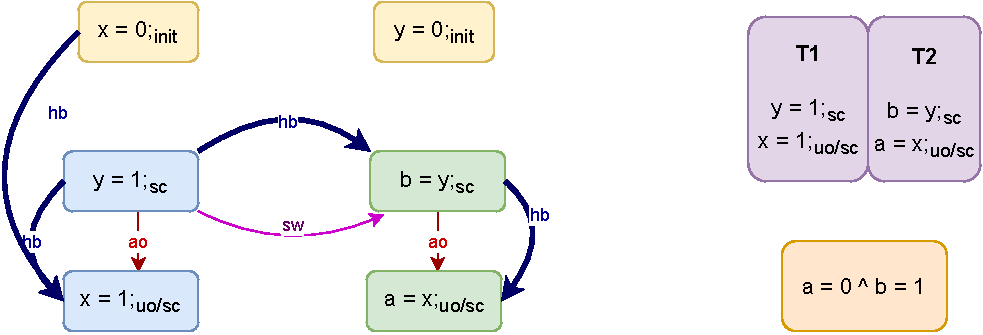
\includegraphics[scale=0.7]{InstructionReordering/Example7R(Wuo,sc-Wsc).pdf}
            \caption{Case where events of T1 are reordered, resulting in  a = 0 and b = 1 to be valid.}
        \end{figure}
        
        The figure on the right above shows the program after reordering the two events in $T1$ where case of reads in the orange box is possible. 
        The figure on the left shows the Candidate Execution that explains the orange box case. 
        Observations:
        \begin{itemize}
            \item From the Candidate Execution, we can infer $\neg\reln{x=1_{uo/sc}}{hb}{a=x_{uo/sc}}$
            \item Hence, there is no pattern that the Axioms restrict, thus validating $x$ to be read as $0$ by $a$. 
        \end{itemize}

        \critic{purple}{All the above shown counter examples only rely on the axiom of coherent reads to show that it is not safe to do the reordering. Does it mean that whenever SC-Atomics axiom can be triggered, Coherent Reads also can be triggered? Investigate this.}

        \critic{red}{All the above counter examples have a lot of repetitive text and can have better formal arguments than a list of observations. Make plans to clean up this once filled in with all the counter examples.}


